% Creating a simple Title Page in Beamer
\documentclass{beamer}

% Theme choice:
\usetheme{AnnArbor}

% Change numbers style
\usepackage{enumitem}

% customize the caption
\setbeamerfont{caption}{size=\large}
\setbeamercolor{caption}{fg=blue}
\setbeamercolor{caption name}{fg=red}

% Title page details:
\title{Introduction to Topology}
\author{yuzuki}
\institute{Eyes, Japan}
\date{\today}
\logo{

\includegraphics[width=3cm]{eyes-japan-logo.png}
}

\begin{document}

% Title page frame
\begin{frame}
    \titlepage
\end{frame}

% Outline frame
\begin{frame}{Outline}
    \tableofcontents
\end{frame}

% Current section
\AtBeginSection[ ]
{
\begin{frame}{Outline}
    \tableofcontents[currentsection]
\end{frame}
}

% Presentation structure
\section{Euler's theorem}

\begin{frame}{Euler's theorem}
\begin{columns}
% Column 1
\begin{column}{0.5\textwidth}
  \begin{block}{}
    \begin{itemize}
    \item v: The number of vertices.
    \item e: The number of edges.
    \item f: The number of faces.
    \end{itemize}
  \end{block}
  \begin{block}{}
    $v - e + f = 2$
  \end{block}
  \begin{block}{}
    \begin{itemize}
    \item convex
    \item not convex
    \end{itemize}
  \end{block}
\end{column}
% Column 2
\begin{column}{0.5\textwidth}
    \begin{figure}
    \centering
        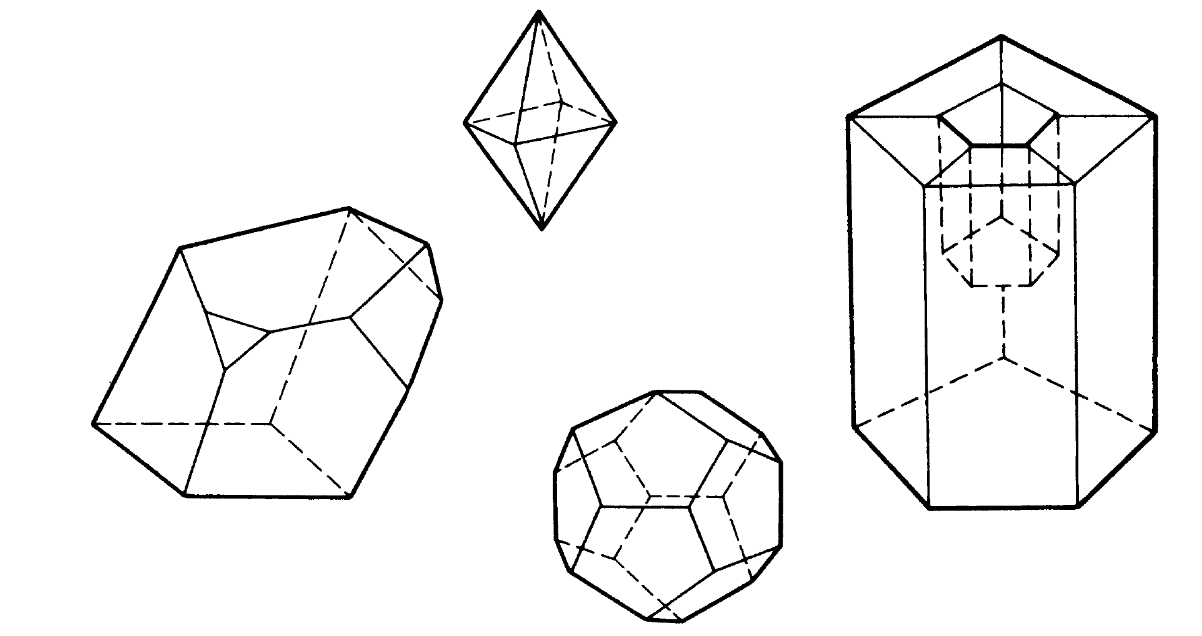
\includegraphics[width=0.7\textwidth]{figure_1_1.png}
        \caption{Polyhedra}
    \end{figure}
\end{column}
\end{columns}
\end{frame}

\begin{frame}{Euler's theorem}
\begin{columns}
% Column 1
\begin{column}{0.5\textwidth}
  \begin{block}{}
    \begin{itemize}
    \item A polyhedron whose surface consists of two distinct pieces.
    \item Its surface is not connected.
    \item Each of the pieces of surface contributes 2 to $v - e + f$.
    \end{itemize}
  \end{block}
  \begin{block}{}
    $v - e + f = 4$
  \end{block}
\end{column}
% Column 2
\begin{column}{0.5\textwidth}
    \begin{figure}
    \centering
        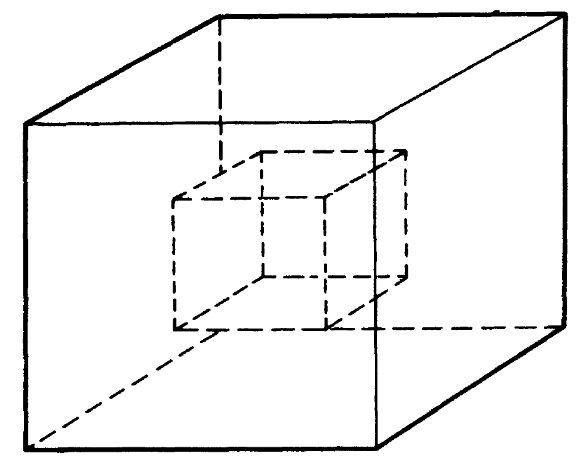
\includegraphics[width=0.7\textwidth]{figure_1_2.png}
        \caption{A cube with a small cube removed from its interior}
    \end{figure}
\end{column}
\end{columns}
\end{frame}

\begin{frame}{Euler's theorem}
\begin{columns}
% Column 1
\begin{column}{0.5\textwidth}
  \begin{block}{}
    \begin{itemize}
    \item A polyhedron whose surface consists of all one piece.
    \item Can find a loop on the surface which does not separate it into two distinct parts.
    \item Imagine: Cutting round the loop with a pair of scissors, then the surface does not fall into two pieces.
    \end{itemize}
  \end{block}
  \begin{block}{}
    $v - e + f = 0$
  \end{block}
\end{column}
% Column 2
\begin{column}{0.5\textwidth}
    \begin{figure}
    \centering
        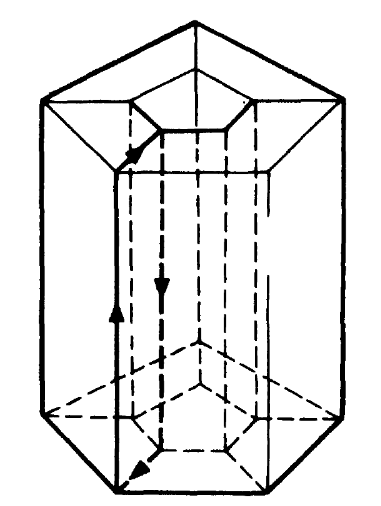
\includegraphics[width=0.7\textwidth]{figure_1_3.png}
        \caption{A prism with a hole straight through the centre}
    \end{figure}
\end{column}
\end{columns}
\end{frame}

\begin{frame}{Euler's theorem}
\begin{columns}
% Column 1
\begin{column}{0.4\textwidth}
  \begin{block}{}
    \begin{itemize}
    \item The surfaces of solids(except, that is, when we mentioned convexity).
    \item Use the word polyhedron for such a surface, rather than for the solid which it bounds.
    \item A \textsl{polyhedron} is a finite collection of plane polygons which fit together nicely in the rigth sense:
    \end{itemize}
  \end{block}
\end{column}
% Column 2
\begin{column}{0.6\textwidth}
  \begin{block}{}
    \begin{itemize}
    \item If two polygons meet they do so in a common edge, and each edge of a polygon lies in precisely one other polygon.
    \item In addition, we ask that if we consider the polygons which contain a particular vertex, then we can label them $Q_1$, $Q_2$,....,$Q_k$ in such a way that $Q_i$ has an edge in common with $Q_{i+1}$ for $1 <= i < k$, and $Q_k$ has an edge in common with $Q_1$.
    \item In other words, the polygons fit together to form a piece of surface around the given vertex (The number \textsl{k} may vary from one vertex to another).
    \end{itemize}
  \end{block}
\end{column}
\end{columns}
\end{frame}

\begin{frame}{Euler's theorem}
% Theorem environment
\begin{theorem}[Euler's theorem.]
  Let P be a polyhedron which satisfies:
  \begin{enumerate}[label={(\alph*)}]
    \item Any two vertices of P can be connected by a chain of edges.
    \item Any loop on P which is made up of straight line segments (not necessary edges) separates P into two pieces.
  \end{enumerate}
  Then v - e + f = 2 for P.
\end{theorem}
\end{frame}

\begin{frame}{Euler's theorem}
\begin{columns}
% Column 1
\begin{column}{0.5\textwidth}
  \begin{definition}[Graph]
    A connected set of vertices and edges of \textsl{P}.
    \begin{itemize}
    \item Connected simply means that any two vertices can be joined by a chain of edges in the graph.
    \item We use the word graph for any finite connected set of line segments in 3-space which fit together nicely as the right figure.
    \item If two segments intersect they are required to do so in a common vertex.
    \end{itemize}
  \end{definition}
\end{column}
% Column 2
\begin{column}{0.5\textwidth}
    \begin{figure}
    \centering
        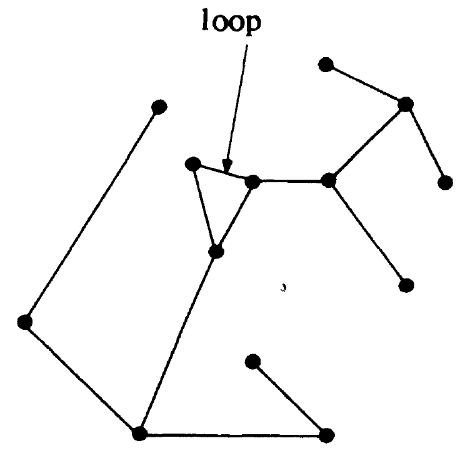
\includegraphics[width=0.7\textwidth]{figure_1_4_b.png}
        \caption{Graph}
    \end{figure}
\end{column}
\end{columns}
\end{frame}

\begin{frame}{Euler's theorem}
\begin{columns}
% Column 1
\begin{column}{0.5\textwidth}
  \begin{definition}[Tree]
    A graph which does not contain any loops.
    \begin{itemize}
    \item For a tree, the number of vertices minus the number of edges is equal to 1.
    \item If the tree is denoted by \textsl{T}, we shall write this as $v(T) - e(T) = 1$.
    \end{itemize}
  \end{definition}
\end{column}
% Column 2
\begin{column}{0.5\textwidth}
    \begin{figure}
    \centering
        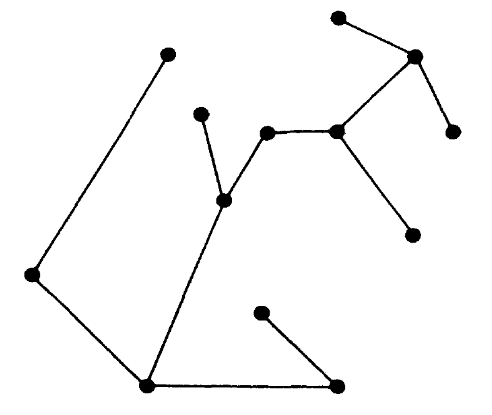
\includegraphics[width=0.7\textwidth]{figure_1_4_a.png}
        \caption{Tree}
    \end{figure}
\end{column}
\end{columns}
\end{frame}

\begin{frame}{Euler's theorem}
\begin{columns}
% Column 1
\begin{column}{0.5\textwidth}
  \begin{proof}
    \begin{itemize}
    \item The set of all vertices and edges of \textsl{P} is a graph.
    \item In any graph find a subgraph which is a tree and which contains all the vertices of the original.
    \item Choose a tree \textsl{T} which consists of some of the edges and all of the vertices of \textsl{P}.
    \end{itemize}
  \end{proof}
\end{column}
% Column 2
\begin{column}{0.5\textwidth}
    \begin{figure}
    \centering
        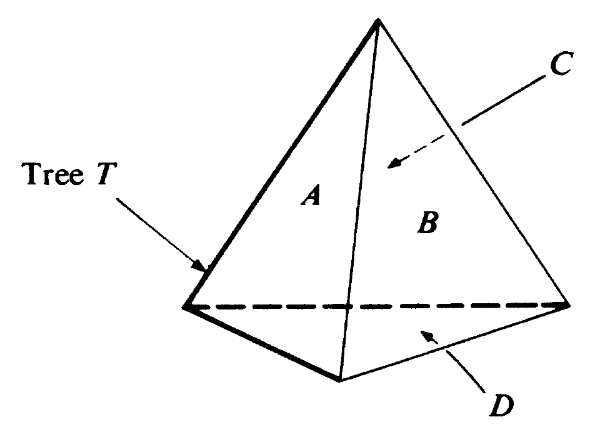
\includegraphics[width=0.7\textwidth]{figure_1_5_a.png}
        \caption{Subgraph-Tree}
    \end{figure}
\end{column}
\end{columns}
\end{frame}

\begin{frame}{Euler's theorem}
\begin{columns}
% Column 1
\begin{column}{0.6\textwidth}
  \begin{proof}
    Form a sort of dual to \textsl{T}. This dual is a grap $\Gamma$ defined as follows:
    \begin{itemize}
    \item For each face \textsl{A} of \textsl{P} we give $\Gamma$ a vertex $\acute{A}$.
    \item Two vertices $\acute{A}$ and $\acute{B}$ of $\Gamma$ are joined by an edge if and only if the corresponding faces \textsl{A} and \textsl{B} of \textsl{P} are adjacent with intersection an edge that is not in \textsl{T}.
    \item The vertex $\acute{A}$ corresponding to an interior point of \textsl{A}.
    \item We allow the edges of $\Gamma$ to be bent.
    \end{itemize}
  \end{proof}
\end{column}
% Column 2
\begin{column}{0.4\textwidth}
    \begin{figure}
    \centering
        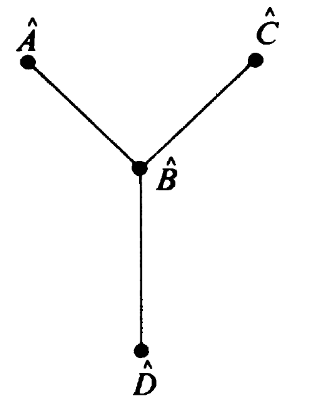
\includegraphics[width=0.7\textwidth]{figure_1_5_b.png}
        \caption{Associated tree $\Gamma$}
    \end{figure}
\end{column}
\end{columns}
\end{frame}

\begin{frame}{Euler's theorem}
\begin{columns}
% Column 1
\begin{column}{0.6\textwidth}
  \begin{proof}
    Dual $\Gamma$ is connected and is therefore a graph.
    \begin{itemize}
    \item Intuitively, if two vertices of $\Gamma$ cannot be connected by a chain of edges of $\Gamma$, then they must be separated from one another by a loop of \textsl{T}.
    \item Since \textsl{T} does not contain any loops we deduce that $\Gamma$ must be connected.
    \end{itemize}
  \end{proof}
\end{column}
% Column 2
\begin{column}{0.4\textwidth}
    \begin{figure}
    \centering
        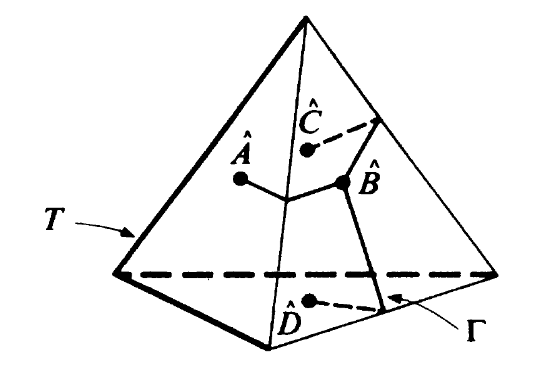
\includegraphics[width=0.7\textwidth]{figure_1_5_c.png}
        \caption{Associated tree $\Gamma$}
    \end{figure}
\end{column}
\end{columns}
\end{frame}

\begin{frame}{Euler's theorem}
\begin{columns}
% Column 1
\begin{column}{0.6\textwidth}
  \begin{proof}
    In fact $\Gamma$ is a tree.
    \begin{itemize}
    \item For if there were a loop in $\Gamma$ it would separate \textsl{P} into two distinct pieces by hypothesis (b), and each if these pieces must contain at least one vertex of $\Gamma$.
    \item Any attempt to connect two vertices of \textsl{T} which lie in different pieces by a chain of edges results in a chain which  meets this separating loop, and therefore in a chain which cannot lie entirely in \textsl{T}.
    \item This contradicts the fact that \textsl{T} is connected. Therefore $\Gamma$ is a tree.
    \end{itemize}
  \end{proof}
\end{column}
% Column 2
\begin{column}{0.4\textwidth}
    \begin{figure}
    \centering
        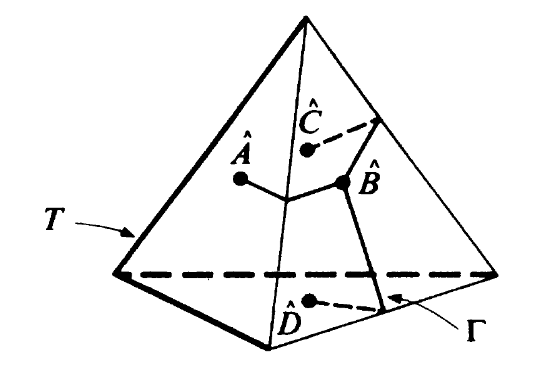
\includegraphics[width=0.7\textwidth]{figure_1_5_c.png}
        \caption{Associated tree $\Gamma$}
    \end{figure}
\end{column}
\end{columns}
\end{frame}

\begin{frame}{Euler's theorem}
\begin{columns}
% Column 1
\begin{column}{0.6\textwidth}
  \begin{proof}
    \begin{itemize}
    \item Since $v(T) - e(T) = 1$ and $v(\Gamma) - e(\Gamma) = 1$.
    \item Therefore $v(T) - [e(T) + e(\Gamma)] + v(\Gamma) = 2$.
    \item By construction $v(T) = v$, $e(T) + e(\Gamma) = e$, $v(\Gamma) = f$.
    \end{itemize}
  \end{proof}
\end{column}
% Column 2
\begin{column}{0.4\textwidth}
    \begin{figure}
    \centering
        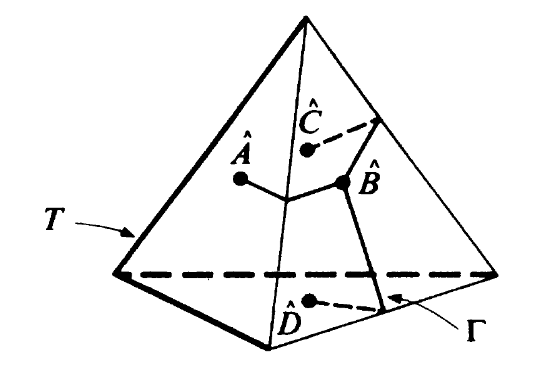
\includegraphics[width=0.7\textwidth]{figure_1_5_c.png}
        \caption{Associated tree $\Gamma$}
    \end{figure}
\end{column}
\end{columns}
\end{frame}

\section{Topological equivalence}
\section{Surfaces}
\section{Abstract spaces}
\section{A classification theorem}

\end{document}